\def\title{Material de Apoyo}
\def\subtitle{Función afín}
\def\curso{Segundo medio}

\documentclass{caes}

\begin{document}

\titulo{Objetivos de la clase}
\begin{itemize}
    \item Establecer metodología para determinar la ecuación de una recta sin usar ayudas gráficas. 
    \item Diferenciar cuando una tabla de puntos corresponde o no a una recta. 
\end{itemize}

\titulo{Ticket de entrada}

\pregunta Determinar la ecuación de la recta que pasa por los puntos:

\def\tabla{%
\begin{mtabla}{}
    x & y \\
    -4 & -7 \\
    8 & 8 \\
\end{mtabla}
}
\begin{center}
    \begin{tikzpicture}
        \node (tabla) {\tabla};
        \node[right=1cm of tabla] (grafica) {\plano[9][9][-9][-9]}; 
    \end{tikzpicture}    
\end{center}

\desarrollo

\pregunta Determinar la ecuación de la recta que pasa por los puntos:

\def\tabla{%
\begin{mtabla}{abovesep=5pt,belowsep=5pt}
    x & y \\
    1 & $-\dfrac{5}{2}$ \\
    2 & $-\dfrac{11}{2}$ \\
\end{mtabla}
}
\def\grafica{%
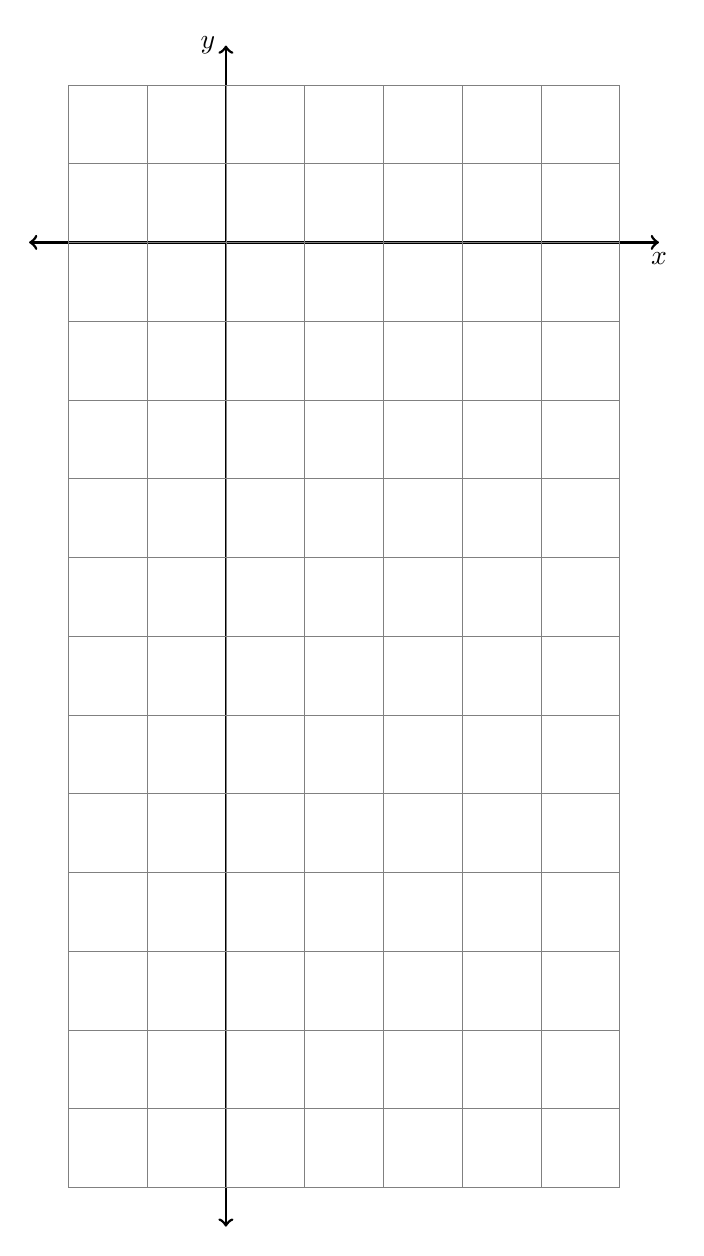
\begin{tikzpicture}[line width=1pt]
    \draw[<->] (-2.5,0) -- (5.5,0) node[below] {$x$};
    \draw[<->] (0,-12.5) -- (0,2.5) node[left] {$y$};
    \draw[help lines] (-2,-12) grid (5,2);
\end{tikzpicture}
}

\begin{center}
    \begin{tikzpicture}
        \node (tabla) {\tabla};
        \node[right=1cm of tabla] (grafica) {\grafica}; 
    \end{tikzpicture}    
\end{center}

\desarrollo[5cm]

\newpage

\titulo{Metodología para encontrar la ecuación de una recta}

\def\formula{%
\begin{tikzpicture}[line width=1pt]
    \draw node[circle,fill, minimum size=7pt,inner sep=0pt, outer sep=0pt,label=left:{$(x_0\,,y_0)$}] {} (0,0) -- node[midway,below=15pt] {$x_1 - x_0$} (3,0) -- node[right=15pt] (dif) {$(y_1 - y_0)$} (3,3) node[minimum size=7pt, inner sep=0pt, outer sep=0pt,circle,fill,label=above:{$(x_1\,,y_1)$}] {} -- (0,0);
    \draw[decorate, decoration={calligraphic brace,mirror,raise=4pt,amplitude=10pt}] (0,0) -- (3,0);
    \draw[decorate, decoration={calligraphic brace,raise=4pt,amplitude=10pt,mirror}] (3,0) -- (3,3);
    %\node (flecha) at (current bounding box.east) {asds};
    \node[right=5mm of dif] (flecha) {\huge$\Rightarrow$};
    \node[right=5mm of flecha] {$m = \dfrac{\text{largo lado vertical}}{\text{largo lado horizontal}} =\dfrac{y_1 - y_0}{x_1 - x_0}$};
\end{tikzpicture}
}
\begin{center}
    \formula
\end{center}

\begin{enumerate}
    \item En el triángulo que se forma entre ambos puntos, calcular el largo del lado horizontal y vertical de la forma:
    \begin{equation*}
        \text{largo lado vertical} = y_1 - y_0 \quad\quad\quad \text{largo lado horizontal} = x_1 - x_0
    \end{equation*}
    \item Calcular la pendiente ($m$) directamente como la división de los largos del lado vertical y el horizontal del triángulo. 
    \begin{equation*}
        m = \dfrac{y_1 - y_0}{x_1 - x_0}
    \end{equation*}
    \item Una vez que se conoce el valor de la pendiente ($m$), se puede encontrar el coeficiente de posición ($n$) 
    despejándolo en la ecuación de la recta ($y=m\cdot x + n$), ya que, se conocen todos los valores de esa ecuación salvo $n$. Es decir:
    \begin{equation*}
        n = y_0 - m\cdot x_0 \quad \text{o} \quad n = y_1 - m\cdot x_1
    \end{equation*}
    Donde $(x_0\,,y_0)$ y $(x_1\,,y_1)$ son los puntos que se conocen de la función.
\end{enumerate}

\titulo{Ticket de salida}

\pregunta Determinar la ecuación de la recta que pasa por los puntos:

\def\tabla{%
\begin{mtabla}{belowsep=7pt, abovesep=7pt}
    x & y \\
    $\dfrac{1}{3}$ & $\dfrac{3}{5}$ \\
    $\dfrac{1}{2}$ & $\dfrac{7}{10}$ \\
\end{mtabla}
}
\begin{center}
    \tikz \node {\tabla} node[right=2cm] {\Caja[Desarrollo][0.75\linewidth][7cm]};    
\end{center}

\end{document}